Diktat does AST-analysis. This means that for internal representation (IR) it uses Abstract Syntax Tree that was created from the parsed code by the kotlin-compiler.  This chapter describes how diktat works

\subsection{ktlint}
\par
To quickly and efficiently analyze the program code, you first need to transform it into a convenient data structure. This is exactly what ktlint does - it parses plain text code into an abstract syntax tree. In ktlint, this happens in the \textsl{prepareCodeForLinting}\footnote{\url{https://github.com/pinterest/ktlint/blob/master/ktlint-core/src/main/kotlin/com/pinterest/ktlint/core/KtLint.kt}} method. This method uses Kotlin libraries to create a root node of type FILE.

\begin{figure}[H]
  \centering
  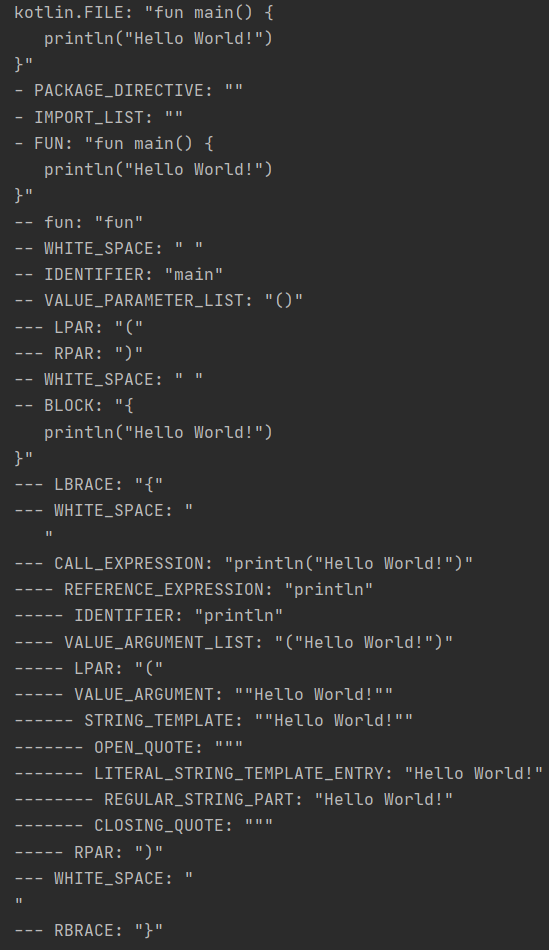
\includegraphics[scale=0.5]{wp/pictures/fileNode.PNG}
  \caption{Example of root Node}   
\end{figure} 

If there are error elements inside the constructed tree, then the corresponding error is displayed. Further, for each rule in the ruleset, the \textsl{visit} method is called to which the root node itself and its “children” are sequentially passed.
At startup, you can pass flags to ktlint - one of them is "-F". This flag means that the rule will not only report an error, but try to fix it.

\subsection{diKTat}
\par
Another feature of ktlint is that at startup you can transfer a JAR file with additional ruleset(s), and then all nodes will be passed to these rules. This is diKTat! DiKTat is a set of easily configurable rules for static code analysis. 
The set of all rules is described in the \textsl{DiktatRuleSetProvider}\footnote{\url{https://github.com/cqfn/diKTat/blob/master/diktat-rules/src/main/kotlin/org/cqfn/diktat/ruleset/rules/DiktatRuleSetProvider.kt}} class. This class overrides the \textsl{get()} method of the \textsl{RuleSetProvider}\footnote{\url{https://github.com/pinterest/ktlint/blob/master/ktlint-core/src/main/kotlin/com/pinterest/ktlint/core/RuleSetProvider.kt}} interface, which returns a set of rules to be "traversed". But before returning this set, the configuration file, in which the user has independently configured all the rules, is read. If there is no configuration file, then a warning will be displayed and the rules will be triggered in according with the default configuration file. 
Each rule must implement the \textsl{visit} method of the abstract Rule class, which describes the logic of the rule.

\begin{figure}[H]
  \centering
  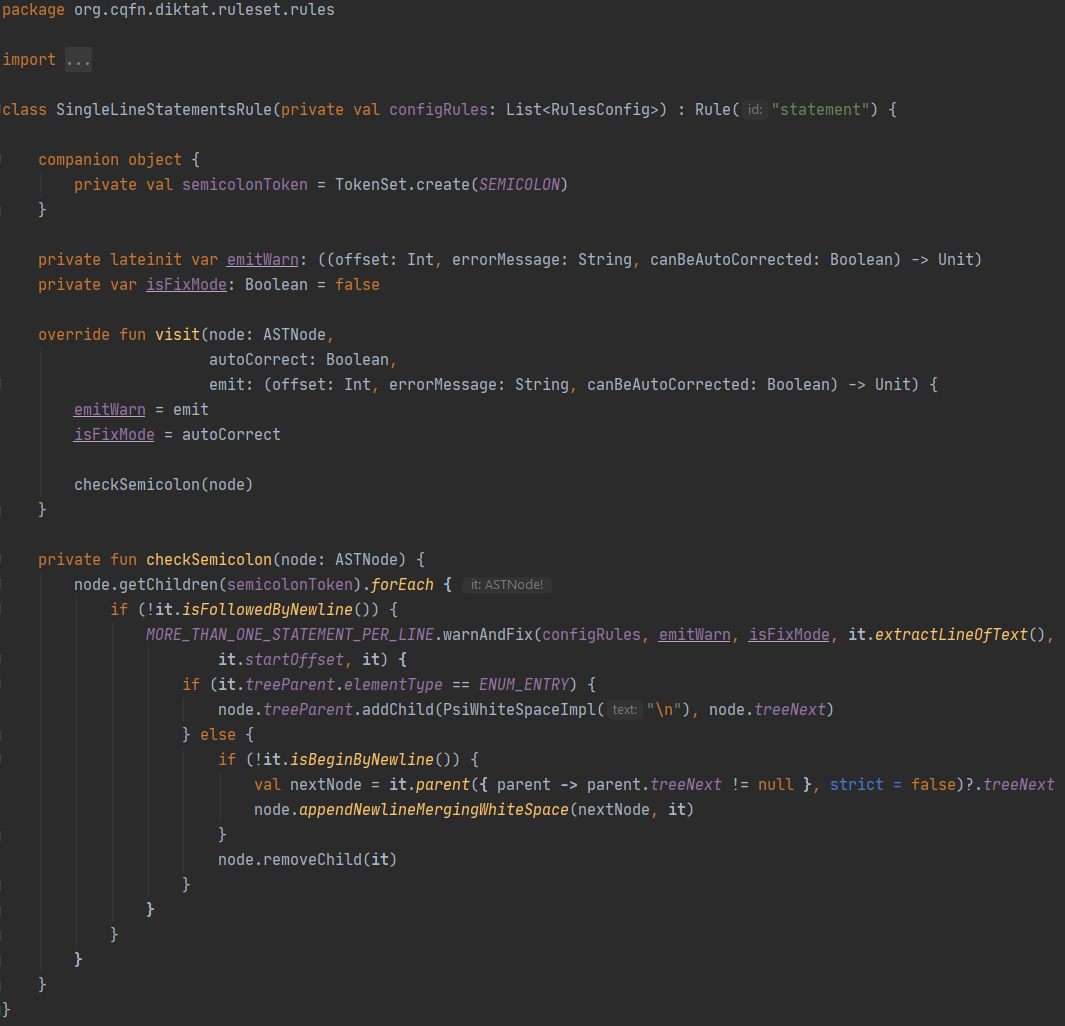
\includegraphics[scale=0.5]{wp/pictures/ruleExample.PNG}
  \caption{Example of rule}   
\end{figure} 

The example above describes the rule in which you cannot write more than two statements on one line. The list of configurations is passed to the parameter of this rule so that the error is displayed only when the rule is enabled (further it will be described how to enable and disable the rule). The class fields and the \textsl{visit} method are described below. The first parameter in method is ASTNode - the node that we got in the parsing in ktlint. Then a check occurs: if the code contains a line in which more than one statement per line and this rule is enabled, then the rule will be executed and, depending on the mode in which the user started ktlint, the rule will either simply report an error or fix it. In our case, when an error is found, the method is called to report and fix the error - \textsl{warnAndFix()}.

\subsection{Examples of unique inspections}
\par
